\documentclass{entcs} 
\usepackage{entcsmacro}
\usepackage{ifxetex}
\ifxetex
\else
\usepackage[utf8]{inputenc}
\fi

\usepackage{amsmath}
\usepackage{mathcomp,amsfonts,amssymb}
\usepackage[authoryear]{natbib}
\usepackage[mathscr]{euscript}
\usepackage{algorithmic,algorithm}
\usepackage{graphicx}
\usepackage{color}
\usepackage{tikz}


\usepackage{enumitem}
\usepackage{dcolumn}

\usepackage{listings}

\newcommand{\abstr}[1]{#1^\sharp}
\newcommand{\parts}[1]{\mathscr{P}(#1)}
\newcommand{\ZZ}{\mathbb{Z}}
\newcommand{\QQ}{\mathbb{Q}}
\newcommand{\RR}{\mathbb{R}}
\newcommand{\widening}{\mathop{\triangledown}}

\def\newblock{\hskip .11em plus .33em minus .07em}

\tikzstyle{arrow}=[->,line width=.05cm,draw=red!90!blue!60!black]

\usetikzlibrary{snakes,arrows,shapes,backgrounds,shadows,automata,patterns}
%\usepgflibrary{snakes}

\tikzstyle{state}=[circle,fill=black!25,minimum size=13pt,inner sep=0pt]
\tikzstyle{rstate}=[rectangle,fill=black!25,minimum size=13pt,inner sep=0pt]
\tikzstyle{transition}=[rectangle,semithick,draw=black!75,
  			  minimum size=4mm]
\tikzstyle{transition2}=[transition,rectangle,thick,dashed,
  			  minimum size=4mm]
\tikzstyle{PRstate}=[circle,double,draw,fill=blue!15,minimum size=13pt,inner sep=0pt]
\tikzstyle{polyhedra}=[blue!25,opacity=0.5,pattern=north west lines,pattern
color=blue]
\tikzstyle{line}=[black,thick]

\lstnewenvironment{C}
{\lstset{language=C,
		basicstyle=\ttfamily,
		commentstyle=\textit,
		showstringspaces=false}}
{}

% The following is enclosed to allow easy detection of differences in
% ascii coding.
% Upper-case    A B C D E F G H I J K L M N O P Q R S T U V W X Y Z
% Lower-case    a b c d e f g h i j k l m n o p q r s t u v w x y z
% Digits        0 1 2 3 4 5 6 7 8 9
% Exclamation   !           Double quote "          Hash (number) #
% Dollar        $           Percent      %          Ampersand     &
% Acute accent  '           Left paren   (          Right paren   )
% Asterisk      *           Plus         +          Comma         ,
% Minus         -           Point        .          Solidus       /
% Colon         :           Semicolon    ;          Less than     <
% Equals        =3D           Greater than >          Question mark ?
% At            @           Left bracket [          Backslash     \
% Right bracket ]           Circumflex   ^          Underscore    _
% Grave accent  `           Left brace   {          Vertical bar  |
% Right brace   }           Tilde        ~

% A couple of exemplary definitions:

\newcommand{\Nat}{{\mathbb N}}
\newcommand{\Real}{{\mathbb R}}
\def\lastname{Henry, Monniaux \& Moy}
\begin{document}
\begin{frontmatter}
  \title{PAGAI : a path sensitive static analyser} 
  \author{Julien Henry \thanksref{imag.fr}}
  \address{Universit\'e Joseph Fourier, VERIMAG\\
    Grenoble, France} 
	\author{David Monniaux\thanksref{imag.fr}}
  \address{CNRS, VERIMAG\\
    Grenoble, France} 
	\author{Matthieu Moy\thanksref{grenoble-inp.fr}}
  \address{Grenoble-INP, VERIMAG\\
    Grenoble, France} 
	
    \thanks[imag.fr]{Email:
    \href{First Name.Last Name@imag.fr} {\texttt{\normalshape
        First Name.Last Name@imag.fr}}} 
    \thanks[grenoble-inp.fr]{Email:
    \href{Matthieu.Moy@grenoble-inp.fr} {\texttt{\normalshape
        Matthieu.Moy@grenoble-inp.fr}}} 
\begin{abstract} 
	We describe the design and the implementation of PAGAI,
        a new static analyzer working over the LLVM compiler infrastructure,
        which computes inductive invariants on the numerical variables of the
        analyzed program.

	PAGAI implements various state-of-the-art algorithms combining abstract
	interpretation and decision procedures (SMT-solving),
        focusing on distinction of paths inside the control flow graph while
        avoiding systematic exponential enumerations.
        It is parametric in the abstract domain in use, the algorithm,
        and the decision procedure.

	We compared the time and precision of various combinations of
	analysis algorithms and abstract domains, with extensive
        experiments both on personal benchmarks and widely available
        GNU programs.
\end{abstract}
\begin{keyword}
	Static Analysis, Program Verification, Abstract Interpretation, Decision
	Procedure, Satisfiability Modulo Theories.
\end{keyword}
\end{frontmatter}
\section{Introduction}\label{intro}
Sound static analysis automatically computes properties on programs, such as the possible values of their variables during execution.
Applications include:
showing that a program has no runtime error (such as arithmetic overflow, division by zero, array access out of bounds), as in e.g. the Astrée analyzer \cite{ASTREE_ESOP05};
computing invariants for use with assisted proof systems (such as the B method, Frama-C\footnote{http://www.frama-c.com/}), thereby lessening the burden on the user;
computing invariants for advanced optimization techniques in compilation (e.g. showing that two array cells are distinct, in order to allow instruction reordering between assignments to these cells).

Abstract Interpretation is a general framework for fully automatic static
analysis, that computes inductive invariants at various control points of an
imperative program. Linear Relation Analysis (LRA) is a direct application of
this framework, that computes an upper-approximation of the set of the reachable
states of a numerical program.

This paper introduces PAGAI, a new tool for static analysis, that
computes numerical invariants at the different control points of a program.
This tool uses the internal representation of LLVM\citep{LLVM_langref,Lattner:2004:LCF:977395.977673},
which is a target for several industrial-strengh compilers, most notably Clang
(supporting C,
C++ and Objective-C) and llvm-gcc (supporting C, C++, Fortran and Ada).
Several other verification tools already use the LLVM framework, such as
Calysto, KLEE, LAV, LLBMC.

Our tool is dedicated to experiment with various combination of analysis techniques
by Abstract Interpretation.
Indeed, depending on the iteration strategy, the choice of the abstract domain,
etc, precision and cost of the analysis may hugely vary. 
We experimentally investigate techniques that take benefits of the improvements in SMT solving
to choose the iteration strategy of the Abstract Interpretation framework.

Our platform allows to compare such state-of-the-art techniques and abstract domains on real life
programs, such as GNU projects.


\section{Motivating Example}

It is well know in abstract interpretation that the least upper bound of two or
more abstract values in the abstract domain 
may induce unrecoverable loss of precision. This operation typically occurs with
if-then-else statements and loops.

An example of program where such a loss of precision occurs is depicted in
Figure \ref{example}. In this program, the loop body has two feasible paths that
are executed alternatively, depending on a variable ``phase''. Such kind of
programs often occur in reactive systems. 
Classical abstract interpretation does not prove that $\lstinline|x| < 100$,
because of the abstract union at control point $n_5$. 
To cope with this problem, an idea is compute disjunctive invariants, i.e a
union of values of the abstract domain. However, the number of terms in the
disjunction may grow exponentially with the number of tests in the program.
A second technique is to distinguish all the paths inside the loop, so that we
compute least upper bounds only at the widening points. In this example, if we
distinguish all the 9 paths of the loop, we prove $\lstinline|x| < 100$. Again,
this path enumeration grows exponentially with the number of tests. In order to
avoid this blowup, we use SMT-solving to keep these paths implicit and to
compute them only if needed.

\begin{figure}[!h]
\begin{minipage}[c]{.49\linewidth}
\begin{C}
int x = 0;
int t = 0;
int phase = 0;

while (t < 100) {
   if (phase == 0) 
      x = x+2;
   if (phase == 1) 
      x = x-1;
   phase = 1-phase;
   t++;
}
assert(x <= 100);
\end{C}
\end{minipage}
\begin{minipage}[c]{.49\linewidth}
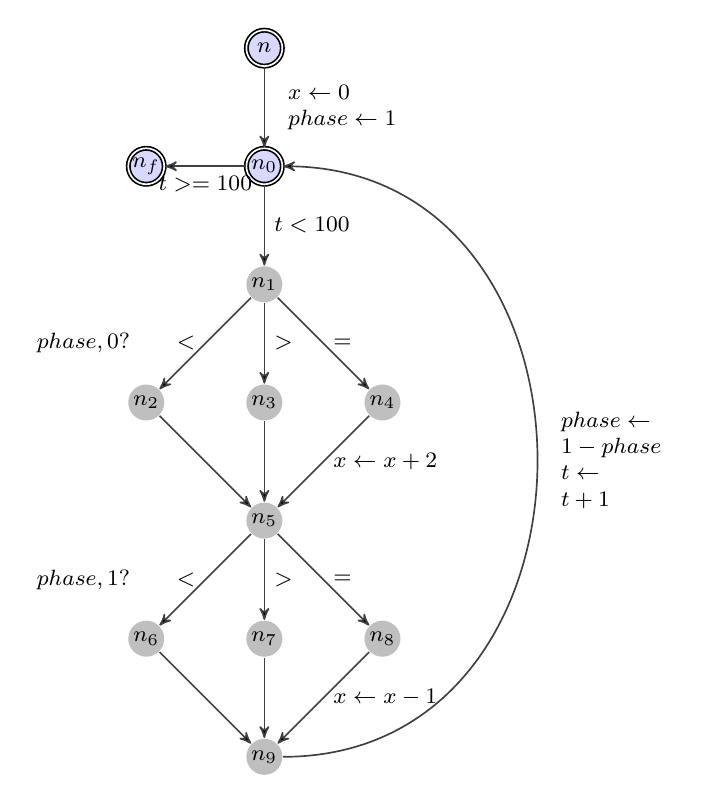
\begin{tikzpicture}[->,>=stealth',auto,node distance=1.5cm,
                    semithick,font=\footnotesize]

	\node[PRstate] (n0) {$n$};
	\node[PRstate] (n00) [below of=n0] {$n_0$};
	\node[PRstate] (nf) [left of=n00] {$n_f$};
	\node[state] (n1) [below of=n00] {$n_1$};
	\node[state] (n3) [below of=n1] {$n_3$};
	\node[state] (n2) [left of=n3] {$n_2$};
	\node[state] (n4) [right of=n3] {$n_4$};
	\node[state] (n5) [below of=n3] {$n_5$};
	\node[state] (n7) [below of=n5] {$n_7$};
	\node[state] (n6) [left of=n7] {$n_6$};
	\node[state] (n8) [right of=n7] {$n_8$};
	\node[state] (n9) [below of=n7] {$n_9$};

  \path [transition] 
		(n0) edge              node  {$\begin{array}{l}
		x \leftarrow 0 \\
		phase \leftarrow 1 
		\end{array}$} (n00);
  \path [transition] 
        (n00)  edge              node {$t>=100$} (nf);
  \path [transition] 
        (n00)  edge              node {$t<100$} (n1);
  \path [transition] 
        (n1) edge			   node [left] {$phase,0?$~ ~ ~ $<$} (n2);
  \path [transition] 
        (n1)  edge              node {$>$} (n3);
  \path [transition] 
        (n1)  edge              node [right] {$=$} (n4);
  \path [transition] 
        (n3) edge              node  {} (n5);
  \path [transition] 
        (n2) edge			   node {} (n5);
  \path [transition] 
        (n4) edge			   node [right] {$x \leftarrow x+2$} (n5);
  \path [transition] 
        (n5) edge			   node [left] {$phase,1?$ ~ ~ ~$<$} (n6);
  \path [transition] 
        (n5) edge			   node {$>$} (n7);
  \path [transition] 
        (n5) edge			   node [right] {$=$} (n8);
  \path [transition] 
        (n6) edge              node {} (n9);
  \path [transition] 
        (n7) edge              node {} (n9);
  \path [transition] 
        (n8) edge              node [right] {$x \leftarrow x-1$} (n9);
  \path [transition] 
        (n9) edge [out=0, in=0, distance=4.3cm] node [right] {
		$\begin{array}{l}
			phase \leftarrow \\
			1-phase \\
			t \leftarrow \\
			t+1
		\end{array}$} (n00);

\end{tikzpicture}
\end{minipage}
\caption{Example of program, where the loop behaviour vary depending on a variable $phase$.}
\label{example}
\end{figure}


\section{Implementation}

PAGAI is a prototype of intraprocedural static analyser, that implements our
recent combined techniques \cite{Henry_Monniaux_Moy_SAS12}
as well as the classical abstract interpretation algorithm, and the state-of-the-art
techniques \emph{Path Focusing} \cite{Monniaux_Gonnord_SAS11} and \emph{Guided
Static Analysis} \cite{DBLP:conf/sas/GopanR07}.

Abstract domains are provided by the APRON library
\citep{DBLP:conf/cav/JeannetM09}, and include convex polyhedra (from the builtin
Polka ``PK'' library), octagons, intervals, and linear congruences. It also has
an interface with the Parma Polyhedra Library (CITATION!!), giving access to
more abstract domains.
For SMT-solving, our analyzer uses Yices
\cite{DBLP:conf/cav/DutertreM06} or Microsoft Z3\cite{DBLP:conf/tacas/MouraB08}
through their C API, and can also operate with any SMT-solver supporting the
SMT-Lib 2 standard \cite{BarST-SMTLIB,BarST-SMT-10} through a pipe.


\begin{table}[!h]
	\tiny
	\centering
\begin{tabular}{|l|r|r|} \hline
	\multicolumn{1}{|c|}{Name} &
        \multicolumn{1}{c|}{kLOC} &
        \multicolumn{1}{c|}{$|P_R|$} \\ \hline
	a2ps & 55 & 2012\\
	gawk & 59 & 902\\ 
	gnuchess & 38 & 1222\\ 
	gnugo & 83 & 2801\\
	grep & 35 & 820\\
	gzip & 27 & 494\\
	lapack/blas & 954 & 16422\\
	make & 34 & 993\\ 
	tar & 73 & 1712\\
	\hline
\end{tabular}
\caption{List of analyzed open-source projects, with their respective number of
lines of code, and their number of control points in $P_R$}
\label{fig:projects}
\end{table}


\subsection{Analysis algorithm}
\label{sec:analysis-algorithm}
For each program, we distinguish a set $P_R = P_W$ of suitable widening points by a simple algorithm: for each procedure, compute the strongly connected components of its control-flow graph using Tarjan's algorithm; the targets of the back-edges of the depth-first search are added to~$P_R$. Note that the resulting set is not necessarily minimal, but is sufficient to disconnect all cycles --- more sophisticated techniques are discussed in e.g. \citet{BourdonclePhd}.

LLVM bitcode is in \emph{static single assignment} (SSA) form: a given scalar variable is given a value at a single syntactic point in the program. In concrete terms, an assignment \lstinline|x=2*x+1;| gets translated into a definition $x_2 = 2x_1+1$, with distinct variables $x_1$ and $x_2$ corresponding to the same original variable \lstinline|x| at different points in the program.
LLVM makes it easy to follow definition-use and use-definition chains: for a given variable (say, $x_2$) one can immediately obtain its definition (say, $2x_1+1$).
One may see conversion to SSA form as a static precomputation of some of the symbolic propagations proposed by \citet{DBLP:conf/vmcai/Mine06} to enhance the precision of analyses.

SSA introduces $\phi$-functions at the head of a control code to define variables whose value depends on which incoming edge to this control node was last taken. For instance, for \lstinline|if (...) { x = 2*x+1; } else { x= 0; }|, then $x_2$ is defined as $\phi(2x_1+1,0)$. In this framework, each variable is uniquely defined as an arithmetic ($+$, $-$, $\times$, $/$) function of other variables that themselves may not be representable as affine linear functions, because they are defined using $\phi$-functions, bitwise arithmetic, loads from memory, or return values from function calls.

This motivates a key implement decision of our tool: only those variables
$v_1,\dots,v_n$ that are not defined by arithmetic operations are retained as
coordinates in the abstract domain (e.g. as dimensions in polyhedra), assuming
they are live at the associate control point. 

	For instance, assume that $x,y,z$ are numerical variables of a program,
	$x$ is defined as $x = y+z$, and $x,y,z$ are live at point $p$. Instead of having
	$x$ as a dimension for the abstract value at point $p$, we only have $y$ and $z$. All the properties
	for $x$ can be directly extracted from the abstract value attached to $p$ and the information $x=y+z$.
	This is an optimisation in the sense that there is redundant information in
	the abstract value if both $x,y$ and $z$ are dimensions of $X_p$.

	Then, classical definition of liveness can be adapted in our case:

	\begin{definition}[Liveness by linearity]
	A variable $v$ is \emph{live by linearity} at a control point $p$ if and
	only if one of these conditions holds:
		\begin{itemize}
		\item $v$ is live in $p$.
		\item There is a variable $v'$, defined as a linear combination of other
		variables $v_1, v_2, \dots, v_n$, so that $\exists i \in \{1,\dots,n\}, v = v_i$,
		and $v'$ is live by linearity in $p$.
		\end{itemize}
	\end{definition}

	Finally, a variable is a dimension in the abstract domain if and only if it
	is live by linearity and it is not defined as a linear combination of
	program variables.

A basic block of code therefore amounts to a \emph{parallel assignment} operation
$(v_1,\dots,v_n) \allowbreak\mapsto\allowbreak
(f_1(v_1,\dots,v_n), \allowbreak, \dots, \allowbreak
 f_n(v_1,\dots,v_n))$;
such operations are directly supported by APRON. This has three benefits:
(i) it limits the number of dimensions in the abstract values, since polyhedra libraries typically perform worse with higher dimensions;
(ii) the abstract operation for a single path in path-focusing methods also is a (large) parallel assignment;
(iii) as suggested by \citet{DBLP:conf/vmcai/Mine06}, this approach is more precise than running abstract operations for each program line separately:
for instance, for \lstinline|y=x; z=x-y;| with precondition $x \in [0,1]$, a line-by-line interval analysis obtains $y \in [0,1]$ and $z \in [-1,1]$ while our ``en bloc'' analysis symbolically simplifies $z = x - x = 0$ and thus $z \in [0,0]$.

In the event that a node is reachable only by a single control-flow edge (which may occur because of dead code, or during the first phases of guided static analysis), the $\phi$ operation reduces to a copy of the values flowing from that edge. In this case, our tool just propagates symbolic values through the predecessor node, without introducing $\phi$-variables.

\subsection{Use}

PAGAI takes as input an LLVM bitcode file, and outputs an inductive invariant
for each control point in $P_R$ (typically, the widening points).
When a program contains \emph{assert} function call, PAGAI also outputs whether
the statement has been proved.
It is also possible to add some preconditions about the variables, etc, using a
function \emph{assume}.
\subsection{Limitations of the tool}

Our tool currently only operates over scalar variables from the SSA representation and thus cannot directly cope with arrays or memory accessed through pointers. We therefore run it after the ``memory to registers'' (\texttt{mem2reg}) optimization phase in LLVM, which lifts most memory accesses to scalar variables.
The remaining memory accesses are treated as undefined values, as are the return
values of function calls. For better precision, we also apply function inlining
to the program, and we unroll every loop once.

Our tool currently assumes that integer variables are unbounded mathematical integers ($\ZZ$) and floating-point variables are real (or rational) numbers. Techniques for sound analysis of bounded integers, including with wraparound, and of floating-point operations have been developed in e.g. the Astr\'ee system \citep{ASTREE_ESOP05,ASTREE_PLDI03}, but porting these techniques to our iteration schemes using SMT-solving requires supplemental work.

Our implementation of path-focusing currently does not use true acceleration
techniques, as proposed by \citet{Monniaux_Gonnord_SAS11}. Instead, it simply runs widening and narrowing iterations on a single path.
The analysis is currently only forward, even though nothing in the techniques
implemented is specific to forward analysis.

\section{Experiments}
\label{sec:experiments}

We conducted extensive experiments on real-life programs in order to compare the
different techniques, mostly on open-source projects (Fig.~\ref{fig:projects}) written in C, C++ and Fortran.

\subsection{Precision of the various techniques}
\label{sec:compare_techniques}

\begin{figure}[h]
  \begin{center}
    % GNUPLOT: LaTeX picture with Postscript
\begingroup
  \makeatletter
  \providecommand\color[2][]{%
    \GenericError{(gnuplot) \space\space\space\@spaces}{%
      Package color not loaded in conjunction with
      terminal option `colourtext'%
    }{See the gnuplot documentation for explanation.%
    }{Either use 'blacktext' in gnuplot or load the package
      color.sty in LaTeX.}%
    \renewcommand\color[2][]{}%
  }%
  \providecommand\includegraphics[2][]{%
    \GenericError{(gnuplot) \space\space\space\@spaces}{%
      Package graphicx or graphics not loaded%
    }{See the gnuplot documentation for explanation.%
    }{The gnuplot epslatex terminal needs graphicx.sty or graphics.sty.}%
    \renewcommand\includegraphics[2][]{}%
  }%
  \providecommand\rotatebox[2]{#2}%
  \@ifundefined{ifGPcolor}{%
    \newif\ifGPcolor
    \GPcolorfalse
  }{}%
  \@ifundefined{ifGPblacktext}{%
    \newif\ifGPblacktext
    \GPblacktexttrue
  }{}%
  % define a \g@addto@macro without @ in the name:
  \let\gplgaddtomacro\g@addto@macro
  % define empty templates for all commands taking text:
  \gdef\gplbacktext{}%
  \gdef\gplfronttext{}%
  \makeatother
  \ifGPblacktext
    % no textcolor at all
    \def\colorrgb#1{}%
    \def\colorgray#1{}%
  \else
    % gray or color?
    \ifGPcolor
      \def\colorrgb#1{\color[rgb]{#1}}%
      \def\colorgray#1{\color[gray]{#1}}%
      \expandafter\def\csname LTw\endcsname{\color{white}}%
      \expandafter\def\csname LTb\endcsname{\color{black}}%
      \expandafter\def\csname LTa\endcsname{\color{black}}%
      \expandafter\def\csname LT0\endcsname{\color[rgb]{1,0,0}}%
      \expandafter\def\csname LT1\endcsname{\color[rgb]{0,1,0}}%
      \expandafter\def\csname LT2\endcsname{\color[rgb]{0,0,1}}%
      \expandafter\def\csname LT3\endcsname{\color[rgb]{1,0,1}}%
      \expandafter\def\csname LT4\endcsname{\color[rgb]{0,1,1}}%
      \expandafter\def\csname LT5\endcsname{\color[rgb]{1,1,0}}%
      \expandafter\def\csname LT6\endcsname{\color[rgb]{0,0,0}}%
      \expandafter\def\csname LT7\endcsname{\color[rgb]{1,0.3,0}}%
      \expandafter\def\csname LT8\endcsname{\color[rgb]{0.5,0.5,0.5}}%
    \else
      % gray
      \def\colorrgb#1{\color{black}}%
      \def\colorgray#1{\color[gray]{#1}}%
      \expandafter\def\csname LTw\endcsname{\color{white}}%
      \expandafter\def\csname LTb\endcsname{\color{black}}%
      \expandafter\def\csname LTa\endcsname{\color{black}}%
      \expandafter\def\csname LT0\endcsname{\color{black}}%
      \expandafter\def\csname LT1\endcsname{\color{black}}%
      \expandafter\def\csname LT2\endcsname{\color{black}}%
      \expandafter\def\csname LT3\endcsname{\color{black}}%
      \expandafter\def\csname LT4\endcsname{\color{black}}%
      \expandafter\def\csname LT5\endcsname{\color{black}}%
      \expandafter\def\csname LT6\endcsname{\color{black}}%
      \expandafter\def\csname LT7\endcsname{\color{black}}%
      \expandafter\def\csname LT8\endcsname{\color{black}}%
    \fi
  \fi
  \setlength{\unitlength}{0.0500bp}%
  \begin{picture}(5040.00,5040.00)%
    \gplgaddtomacro\gplbacktext{%
      \csname LTb\endcsname%
      \put(594,966){\makebox(0,0)[r]{\strut{} 0}}%
      \put(594,1442){\makebox(0,0)[r]{\strut{} 2}}%
      \put(594,1918){\makebox(0,0)[r]{\strut{} 4}}%
      \put(594,2394){\makebox(0,0)[r]{\strut{} 6}}%
      \put(594,2871){\makebox(0,0)[r]{\strut{} 8}}%
      \put(594,3347){\makebox(0,0)[r]{\strut{} 10}}%
      \put(594,3823){\makebox(0,0)[r]{\strut{} 12}}%
      \put(594,4299){\makebox(0,0)[r]{\strut{} 14}}%
      \put(594,4775){\makebox(0,0)[r]{\strut{} 16}}%
      \put(1216,834){\rotatebox{-45}{\makebox(0,0)[l]{\strut{}G/S}}}%
      \put(1705,834){\rotatebox{-45}{\makebox(0,0)[l]{\strut{}PF/S}}}%
      \put(2195,834){\rotatebox{-45}{\makebox(0,0)[l]{\strut{}PF/G}}}%
      \put(2685,834){\rotatebox{-45}{\makebox(0,0)[l]{\strut{}G+PF/PF}}}%
      \put(3174,834){\rotatebox{-45}{\makebox(0,0)[l]{\strut{}G+PF/G}}}%
      \put(3664,834){\rotatebox{-45}{\makebox(0,0)[l]{\strut{}G+PF/S}}}%
      \put(4153,834){\rotatebox{-45}{\makebox(0,0)[l]{\strut{}DIS/G+PF}}}%
      \put(236,2871){\rotatebox{-270}{\makebox(0,0){\strut{}percentage of control points}}}%
    }%
    \gplgaddtomacro\gplfronttext{%
      \put(3656,4602){\makebox(0,0)[r]{\strut{}$\subsetneq$}}%
      \put(3656,4382){\makebox(0,0)[r]{\strut{}$\supsetneq$}}%
      \put(3656,4162){\makebox(0,0)[r]{\strut{}uncomparable}}%
    }%
    \gplbacktext
    \put(0,0){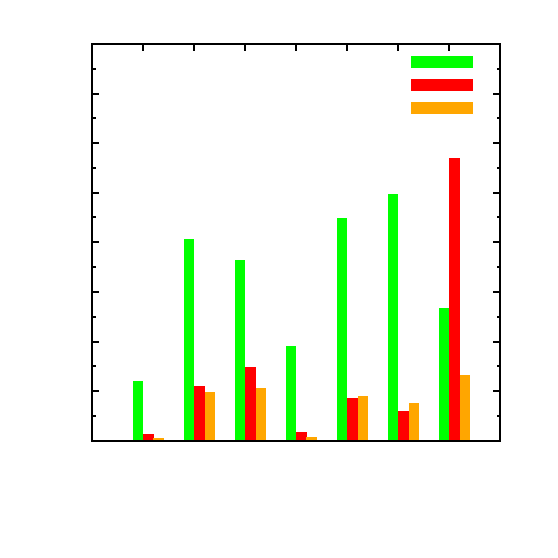
\includegraphics{gnuplot/techniques}}%
    \gplfronttext
  \end{picture}%
\endgroup

  \end{center} 
  \vspace{-20pt}
  \caption{Comparison of the abstract values obtained by classical abstract
  interpretation (S), \emph{Guided Static
  Analysis} (G), \emph{Path-focused} technique (PF), our combined technique
  (G+PF), and its version with disjunctive invariants (DIS).
  The $\subsetneq$ bars gives the percentage of invariants stronger (more precise; smaller with respect to inclusion) with the left-side technique,
$\supsetneq$ the percentage of invariants stronger with the right-side technique,
and ``uncomparable'' gives the percentage of invariants that are uncomparable, i.e
neither greater nor smaller;
the code points where both invariants are equal make up the remaining percentage. See Tab.~\ref{tab:techniques} for details.}
  \label{fig:techniques}
\end {figure}


\begin{table*}
	\tiny
\begin{center}
\setlength{\tabcolsep}{0.75ex}
\begin{tabular}{|l
|D{.}{.}{2}D{.}{.}{2}D{.}{.}{2}%
|D{.}{.}{2}D{.}{.}{2}D{.}{.}{2}%
|D{.}{.}{2}D{.}{.}{2}D{.}{.}{2}%
|D{.}{.}{2}D{.}{.}{2}D{.}{.}{2}%
|D{.}{.}{2}D{.}{.}{2}D{.}{.}{2}%
|D{.}{.}{2}D{.}{.}{2}D{.}{.}{2}|} \hline
\multicolumn{1}{|c|}{\textbf{Benchmark}}
& \multicolumn{3}{c|}{\textbf{G/S}}
& \multicolumn{3}{c|}{\textbf{PF/S}}
& \multicolumn{3}{c|}{\textbf{PF/G}}
& \multicolumn{3}{c|}{\textbf{G+PF/PF}}
& \multicolumn{3}{c|}{\textbf{G+PF/G}}
& \multicolumn{3}{c|}{\textbf{DIS/G+PF}} \\ %\cline{2-16}
& \multicolumn{1}{c}{$\subsetneq$} & \multicolumn{1}{c}{$\supsetneq$} & \multicolumn{1}{c|}{unc.}
& \multicolumn{1}{c}{$\subsetneq$} & \multicolumn{1}{c}{$\supsetneq$} & \multicolumn{1}{c|}{unc.}
& \multicolumn{1}{c}{$\subsetneq$} & \multicolumn{1}{c}{$\supsetneq$} & \multicolumn{1}{c|}{unc.}
& \multicolumn{1}{c}{$\subsetneq$} & \multicolumn{1}{c}{$\supsetneq$} & \multicolumn{1}{c|}{unc.}
& \multicolumn{1}{c}{$\subsetneq$} & \multicolumn{1}{c}{$\supsetneq$} & \multicolumn{1}{c|}{unc.}
& \multicolumn{1}{c}{$\subsetneq$} & \multicolumn{1}{c}{$\supsetneq$} & \multicolumn{1}{c|}{unc.} \\
 \hline
 a2ps-4.14 & .28 & 0 & 0 & 4.82 & 2.55 & 2.27 & 4.54 & 2.55 & 2.27 & 6.81 & .28 & 0 & 8.23 & 0 & 0 & 13.06 & 3.40 & .56 \\ \hline
gawk-4.0.0 & 4.62 & 0 & 0 & 3.70 & 20.37 & .92 & .92 & 22.22 & 0 & 22.22 & 0 & 0 & 11.11 & 2.77 & 0 & 16.66 & 2.77 & .92 \\ \hline
gnuchess-6.0.0 & 1.51 & 3.47 & 0 & 6.50 & 4.33 & 0 & 6.72 & 3.25 & .21 & 6.72 & 2.38 & 0 & 10.19 & 2.38 & 0 & 15.18 & 2.81 & 3.03 \\ \hline
gnugo-3.8 & .51 & 4.44 & .34 & 11.45 & 4.27 & 3.07 & 12.13 & 4.27 & 2.73 & 10.25 & 3.07 & 2.05 & 17.77 & 3.76 & .34 & 9.05 & 11.28 & 4.78 \\ \hline
grep-2.9 & 0 & 6.19 & .47 & 1.90 & 4.76 & .47 & 3.80 & 1.90 & 1.90 & 7.61 & 2.38 & 0 & 8.57 & 2.38 & 0 & 10.47 & 5.23 & .47 \\ \hline
gzip-1.4 & .58 & 7.01 & 1.75 & 1.75 & 12.86 & 1.16 & 3.50 & 8.18 & 1.16 & 15.78 & 2.92 & 1.16 & 17.54 & 1.75 & 0 & 17.54 & 15.78 & 1.16 \\ \hline
lapack-3.3.1 & 2.60 & 5.77 & .40 & 3.11 & 5.06 & 1.03 & 4.66 & 3.47 & 1.62 & 7.55 & 1.06 & 0 & 9.24 & 1.06 & .81 & 16.11 & 7.09 & 1.34 \\ \hline
make-3.82 & 2.61 & .52 & 0 & 1.82 & 6.26 & 1.82 & 1.56 & 8.09 & 1.82 & 11.74 & .52 & 0 & 6.52 & 2.34 & 1.56 & 12.27 & 4.43 & .78 \\ \hline
tar-1.26 & 4.53 & 3.27 & 0 & 5.28 & 2.77 & 0 & 2.77 & 2.01 & .75 & 7.05 & .50 & 0 & 7.05 & .25 & 0 & 9.82 & 7.05 & 1.51 \\ \hline

\end{tabular}
\end{center}
\caption{Result of the comparison of the various techniques described in this
paper: classic Abstract Interpretation (S), \emph{Guided Static Analysis} (G),
\emph{Path-focusing} (PF), our combined technique (G+PF), and its version using
disjunctive invariants (DIS). For
instance, \textbf{G/S} compares the benefits of \emph{Guided Static Analysis}
over the classic Abstract interpretation algorithm.
$\subsetneq$, $\supsetneq$ and ``unc.'' are defined as in Fig.~\ref{fig:techniques}.}
\label{tab:techniques}
\end{table*}

For each program and each pair $(T_1,T_2)$ of analysis techniques, we list
the proportion of control points in $P_R$ where $T_1$ (resp.~$T_2$) gives a
strictly stronger invariant, denoted by $\subsetneq$ (resp. $\supsetneq$),
and the proportion of control points where the invariants given by $T_1$ and
$T_2$ are uncomparable for the inclusion ordering (the remainder of the
control points are thus those for which both techniques give the same
invariant). We use convex polyhedra as the abstract domain.

Let us briefly comment the results given in more details in Table~\ref{tab:techniques} and Figure~\ref{fig:techniques}.
\emph{Guided Static Analysis} from \citet{DBLP:conf/sas/GopanR07} improves the
result of the classical Abstract Interpretation in $2.72\%$ of the control points
in $P_R$.
\emph{Path-focusing} from \citet{Monniaux_Gonnord_SAS11} gives
statistically better results, and finds better invariants than \emph{Guided
Static Analysis} in $9.89\%$ of the cases. However, it also loses precision in an
important number ($2.68\%$) of control points.
Finally, our combined technique gives the most promising results, since it is
statistically more precise than the other techniques.

The analysis using disjunctive invariants greatly improves the
precision of the analysis (for $12.06\%$ of the control points in $P_R$), at an
acceptable time cost (see Table \ref{tab:time}).

While experiencing with techniques that use SMT-solving, we encountered some
limitations due to non-linear arithmetic in the analyzed programs. Indeed, 
the SMT-solver is not able to decide the satisfiability of some SMT-formulae
expressing the semantics of non-linear programs. 
In this case, we skipped the functions for which the SMT-solver returned the
``unknown'' result.
This limitation occurred very rarely in our experiments, except for the analysis
of \emph{Lapack/Blas}, where 798 over the 1602 functions have been skipped.
\emph{Lapack/Blas} implements matrix computations, which use floating-point multiplications.

In cases where the formula is expressed in too rich a logic for the SMT-solver to deal with, a number of workarounds are possible, including:
(i) \emph{Linearization}, as per \citet{DBLP:conf/vmcai/Mine06}, which overapproximates nonlinear semantics by linear semantics.
(ii) Replacing the results of nonlinear operations by ``unknown''.
Neither is currently implemented in our tool.

Table \ref{tab:time} gives the execution time of the different analysis
techniques. It is interesting to see that \emph{Guided Static Analysis} and
\emph{Path-focusing} are sometimes faster than the classical
algorithm.
This seems due to the fact that these algorithms start on a small subset
of the graph, and then may need fewer iterations on the complete graph.
The techniques we introduce in this article are slower, but speed is still on the same order of magnitude as the older ones.

\begin{table}[!h]
	\centering \tiny
\begin{tabular}{|l|r|r|r|r|r|} \hline
	\multicolumn{1}{|c|}{Benchmark} &
        \multicolumn{1}{c|}{\textbf{S}} &
        \multicolumn{1}{c|}{\textbf{G}} &
        \multicolumn{1}{c|}{\textbf{PF}} &
        \multicolumn{1}{c|}{\textbf{G+PF}} &
	\multicolumn{1}{c|}{\textbf{DIS}} \\ \hline
	a2ps-4.14 & 46 & 11 & 45 & 127 & 280 \\
gawk-4.0.0 & 54 & 7 & 14 & 34 & 60 \\
gnuchess-6.0.0 & 164 & 21 & 121 & 411 & 1217 \\
gnugo-3.8 & 222 & 36 & 129 & 398 & 942 \\
grep-2.9 & 40 & 14 & 18 & 50 & 177 \\
gzip-1.4 & 60 & 12 & 40 & 123 & 309 \\
lapack-3.3.1 & 594 & 202 & 2769 & 6897 & 11136 \\
make-3.82 & 22 & 8 & 33 & 90 & 173 \\
sed-4.2 & 42 & 9 & 37 & 154 & 371 \\
tar-1.26 & 275 & 40 & 114 & 316 & 722 \\
 \hline
\end{tabular}
\caption{Execution time for each technique, expressed in seconds}
\label{tab:time}
\end{table}


\subsection{Precision of Abstract Domains}
\label{sec:compare_domains}
\begin{table*}
	\tiny
\begin{center}
\setlength{\tabcolsep}{0.75ex}
\begin{tabular}{|l
|D{.}{.}{2}D{.}{.}{2}D{.}{.}{2}%
|D{.}{.}{2}D{.}{.}{2}D{.}{.}{2}%
|D{.}{.}{2}D{.}{.}{2}D{.}{.}{2}%
|D{.}{.}{2}D{.}{.}{2}D{.}{.}{2}%
|D{.}{.}{2}D{.}{.}{2}D{.}{.}{2}%
|D{.}{.}{2}D{.}{.}{2}D{.}{.}{2}|} \hline
\multicolumn{1}{|c|}{\textbf{Benchmark}}
& \multicolumn{3}{c|}{\textbf{PK/OCT}}
& \multicolumn{3}{c|}{\textbf{PK/BOX}}
& \multicolumn{3}{c|}{\textbf{OCT/BOX}}
& \multicolumn{3}{c|}{\textbf{PK/PKEQ}}
& \multicolumn{3}{c|}{\textbf{PK/GRID}}
& \multicolumn{3}{c|}{\textbf{POLY*/POLY}} \\ %\cline{2-16}
& \multicolumn{1}{c}{$\subsetneq$} & \multicolumn{1}{c}{$\supsetneq$} & \multicolumn{1}{c|}{unc.}
& \multicolumn{1}{c}{$\subsetneq$} & \multicolumn{1}{c}{$\supsetneq$} & \multicolumn{1}{c|}{unc.}
& \multicolumn{1}{c}{$\subsetneq$} & \multicolumn{1}{c}{$\supsetneq$} & \multicolumn{1}{c|}{unc.}
& \multicolumn{1}{c}{$\subsetneq$} & \multicolumn{1}{c}{$\supsetneq$} & \multicolumn{1}{c|}{unc.}
& \multicolumn{1}{c}{$\subsetneq$} & \multicolumn{1}{c}{$\supsetneq$} & \multicolumn{1}{c|}{unc.}
& \multicolumn{1}{c}{$\subsetneq$} & \multicolumn{1}{c}{$\supsetneq$} & \multicolumn{1}{c|}{unc.} \\
 \hline
 a2ps-4.14 & 4.56 & 1.39 & 0.22 & 6.86 & 1.38 & 0.44 & 6.28 & 0 & 0 & 28.75 & 0 & 0 & 23.23 & 0 & 0.60 & 3.71 & 0.22 & 0 \\ \hline
gawk-4.0.0 & 6.49 & 0 & 0 & 9.09 & 0 & 0 & 6.49 & 0 & 0 & 27.27 & 0 & 0 & 26.15 & 0 & 1.11 & 3.52 & 0 & 0 \\ \hline
gnuchess-6.0.0 & 4.27 & 2.51 & 0.33 & 6.47 & 2.50 & 0.40 & 6.52 & 1.65 & 0.08 & 36.48 & 0 & 0 & 35.74 & 0 & 0.82 & 2.88 & 1.04 & 0 \\ \hline
gnugo-3.8 & 8.26 & 1.66 & 1.15 & 11.98 & 1.03 & 1.54 & 11.53 & 0.21 & 0.21 & 34.52 & 0 & 0 & 36.46 & 0 & 0.44 & 8.93 & 1.23 & 0.29 \\ \hline
grep-2.9 & 1.60 & 1.77 & 0.88 & 4.98 & 1.06 & 1.60 & 5.69 & 0 & 0 & 27.04 & 0 & 0 & 26.86 & 0 & 0.17 & 2.86 & 0 & 0 \\ \hline
gzip-1.4 & 7.14 & 1.72 & 0.24 & 10.83 & 0.73 & 1.23 & 9.60 & 0 & 0.24 & 32.69 & 0 & 0 & 32.45 & 0 & 0.24 & 6.15 & 1.47 & 0 \\ \hline
lapack-3.3.1 & 24.96 & 1.61 & 5.13 & 54.06 & 0.57 & 5.99 & 58.42 & 0.48 & 1.02 & 64.14 & 0.06 & 0.06 & 62.50 & 0 & 1.63 & 9.55 & 0.24 & 0.01 \\ \hline
make-3.82 & 2.44 & 2.11 & 0.22 & 7.03 & 0.97 & 1.19 & 7.11 & 0.11 & 0 & 31.11 & 0 & 0 & 32.78 & 0 & 0.82 & 4.00 & 0.33 & 0.44 \\ \hline
tar-1.26 & 1.92 & 0.72 & 0.06 & 4.85 & 0.59 & 0.35 & 4.85 & 0.11 & 0 & 25.11 & 0 & 0.05 & 24.57 & 0 & 0.70 & 1.71 & 0.23 & 0.05 \\ \hline

\end{tabular}
\end{center}
\caption{Results of the comparison of the various abstract domains, when using
the same technique (G+PF). We used as abstract domains Convex Polyhedra (PK and
POLY),
Octagons (OCT), intervals (BOX), linear equalities (PKEQ) and linear congruences
(GRID). The last column compares the domain of Convex Polyhedra with the
improved widening operator from \citet{BagnaraHRZ05SCP} (POLY*), and Convex Polyhedra
using the classical widening operator (POLY). POLY and POLY* use the Parma
Polyhedral Library \cite{PPL}.
$\subsetneq$, $\supsetneq$ and ``unc.'' are defined as in Fig.~\ref{fig:techniques}.}
\label{tab:domain}
\end{table*}

For each program and each pair $(D_1,D_2)$ of abstract domains, we compare by
inclusion the invariants of the different control points in $P_R$ (where $P_R$
is defined as in \ref{sec:compare_techniques}).
The main results are given in Table \ref{tab:domain}.

Statistically, the domain of convex polyhedra gives the better results, but
commonly yields weaker invariants than the domains of octagons/intervals;
this is a known weakness of its widening operator~\cite{Monniaux_LeGuen2011}. 
The Octagon domain appears to be much better than intervals; this is
unsurprising since in most programs and libraries, bounds on loop indices are
non constant: they depend on some parameters (array sizes etc.).

The Lapack/Blas benchmarks are unusual compared to the other programs. These libraries perform matrix computations, using nested loops over indices; such programs are the prime target for polyhedral loop optimization techniques and it is therefore unsurprising that polyhedra perform very well over them.

The analysis of linear equalities (PKEQ) performs very fast compared
to other abstract domains, but yields very imprecise invariants:
it only detects relations of the form $\sum_i a_i x_i = C$ where $a_i$ and $C$ are constants.
The comparison between the domain of convex polyhedra and linear congruences
shows the percentage of points where the use of congruences refines the
invariant. This is the case for $1.04\%$ of the control points in $P_R$.

Finally, we evaluated the benefits of the improved version of the widening
operator for convex polyhedra from \citet{BagnaraHRZ05SCP}, compared to the
classical widening. We found that the improved version from
\citet{BagnaraHRZ05SCP} yields more precise invariants for $6.58\%$ of the
control points in $P_R$.

\section{Conclusion and future work}



\phantomsection\addcontentsline{toc}{section}{References} 
	\bibliographystyle{plainnat}
\bibliography{pagai}
\end{document}

% Pour Emacs:
% Local Variables:
% reftex-cite-format: natbib
% End:
